\documentclass[11pt,a4paper]{article}

\usepackage[utf8]{inputenc}
\usepackage[T1]{fontenc}
\usepackage[ngerman]{babel}
\usepackage{amsmath,amssymb}
\usepackage{geometry}
\usepackage{pdfpages}
\geometry{margin=2.5cm}

\begin{document}

% ---------------------------------------------------------------------------
% Page 1: taken verbatim from the original assignment (unchanged).
% ---------------------------------------------------------------------------
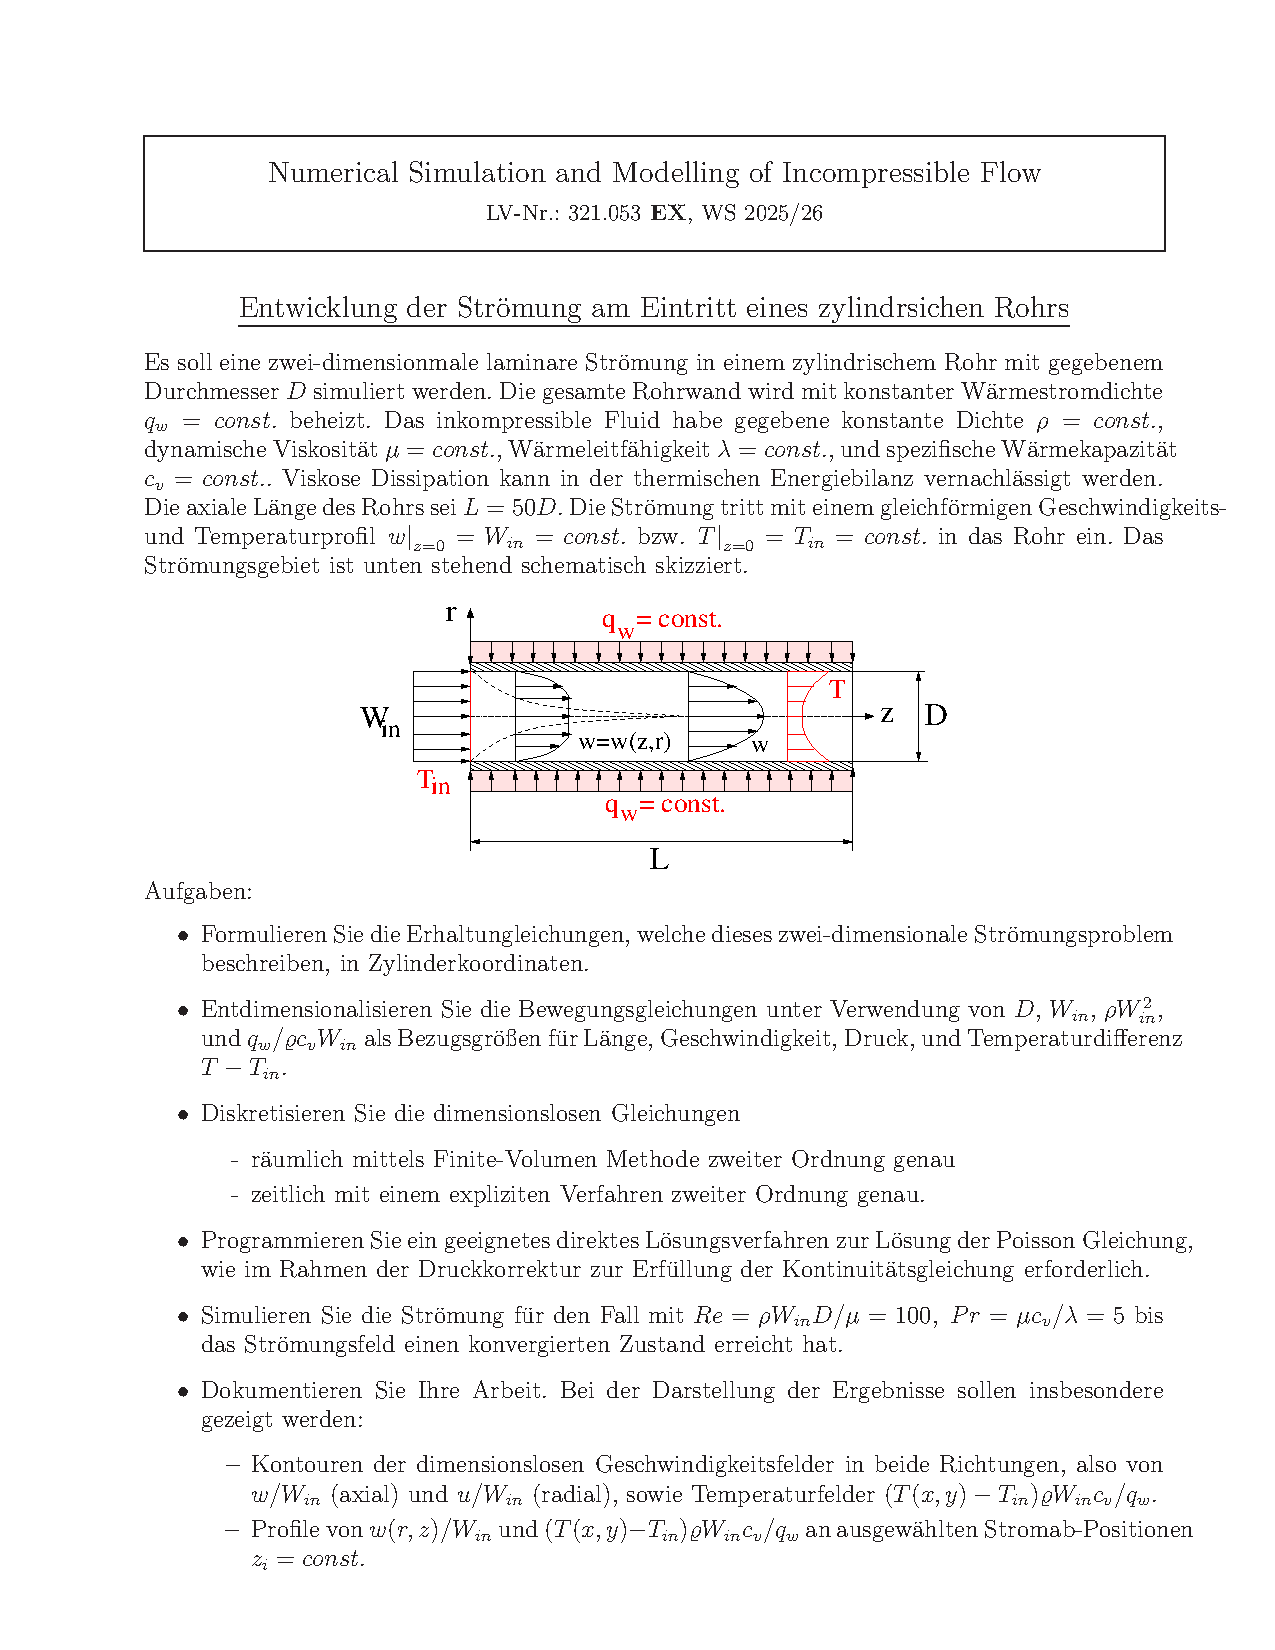
\includepdf[pages=1]{Assignment_WS25_error.pdf}

% ---------------------------------------------------------------------------
% Page 2: corrected. Only the fully-developed comparison temperature profile
% differs from the original page 2 (missing factor 1/2 on Re*Pr in the radial
% terms; additive constant -7/48 instead of -3/4).
% ---------------------------------------------------------------------------
\thispagestyle{empty}

\noindent\fbox{\parbox{\dimexpr\linewidth-2\fboxsep-2\fboxrule\relax}{%
\small
\textbf{Korrigierte Seite~2.} Seite~1 ist unver\"andert. Auf dieser Seite ist \emph{nur} die
voll entwickelte Vergleichs-Temperaturformel berichtigt: in der Originalfassung fehlte der
Faktor $\tfrac12$ vor $Re\,Pr$ in den radialen Termen, und die additive Konstante muss
$-\tfrac{7}{48}$ statt $-\tfrac34$ lauten, damit die Mischtemperatur
$\theta_{\mathrm{bulk}}(z) = 4\,z/D$ f\"ur alle $z\ge 0$ korrekt ist. Die unver\"anderte
Originalfassung liegt als \texttt{Assignment\_WS25\_error.pdf} bei; Herleitung und
Literaturquellen ($Nu = 48/11$) in \texttt{Report/nusselt\_number\_analysis.md}.%
}}

\vspace{2em}

\begin{itemize}
    \item[--] F\"ugen Sie zum Vergleich die Profile f\"ur die voll entwickelte zylindrische
          Rohrstr\"omung hinzu, hier gegeben als
          \begin{align*}
              w &= 2\,W_{\mathrm{in}}\left[\,1 - \left(\frac{2r}{D}\right)^{2}\right], \\[6pt]
              \frac{(T - T_{\mathrm{in}})\,\varrho\, W_{\mathrm{in}}\, c_v}{q_w}
                &= 4\,\frac{z}{D}
                   + Re\,Pr\left[\,\frac{1}{2}\left(\frac{2r}{D}\right)^{2}
                                  - \frac{1}{8}\left(\frac{2r}{D}\right)^{4}
                                  - \frac{7}{48}\,\right],
          \end{align*}
          welche f\"ur zunehmende Laufl\"ange $z$ schlussendlich erreicht werden m\"ussen.
\end{itemize}

\vspace{1em}
\small\noindent
\emph{\"Aquivalente Schreibweise} (Faktor ausgeklammert):
\[
    \frac{(T - T_{\mathrm{in}})\,\varrho\, W_{\mathrm{in}}\, c_v}{q_w}
      = 4\,\frac{z}{D}
        + \frac{1}{2}\,Re\,Pr\left[\left(\frac{2r}{D}\right)^{2}
              - \frac{1}{4}\left(\frac{2r}{D}\right)^{4} - \frac{7}{24}\right].
\]

\end{document}
